%! Author = Johannes Byle
%! Date = 10/17/2021

% Preamble
\documentclass[12pt]{article}
\title{}
\author{Johannes Byle}

% Preamble
\documentclass[12pt]{article}
\title{Math Methods Assignment \#6}
\author{Johannes Byle}


% Packages
\usepackage{amsmath}
\usepackage[margin=0.75in]{geometry}
\usepackage{lipsum}
\usepackage{bbold}
\usepackage{amssymb}
\usepackage{graphicx}
\usepackage{amsmath, amssymb, graphics, setspace}

\newcommand{\mathsym}[1]{{}}
\newcommand{\unicode}[1]{{}}

\newcommand{\p}[2]{\frac{\partial #1}{\partial #2}}
\newcommand{\der}[2]{\frac{d #1}{d #2}}
\newcommand{\curl}{\nabla\times}
\newcommand{\divr}{\nabla\cdot}
% Document
\begin{document}
    \maketitle
    \begin{enumerate}
        \item
        \begin{enumerate}
            \item Starting with Ampere's Law:
            \begin{align*}
                \curl\mathcal{B}&=\frac{4\pi}{c}\pmb{J}+\frac{1}{c}\p{\mathcal{E}}{t}\\
                \divr\left(\nabla\times\mathcal{B}\right)&=\frac{4\pi}{c}\divr\pmb{J}+\frac{1}{c}\p{(\nabla\cdot\mathcal{E})}{t}=0\quad\text{Using the identity: }\nabla\left( \nabla\cdot\times A \right)=0\\
                \divr\left(\nabla\times\mathcal{B}\right)&=\frac{4\pi}{c}\divr\pmb{J}+\frac{4\pi}{c}\p{\rho}{t}=0\quad\text{Using: }\nabla\cdot\mathcal{E}=4\pi\rho\\
                \divr\pmb{J}+\p{\rho}{t}&=0
            \end{align*}
            \item Starting with the curl of the electric field:
            \begin{align*}
                \curl\mathcal{E}&=-\frac{1}{c}\p{\mathcal{B}}{t}\\
                \curl\mathcal{E}&=-\frac{1}{c}\p{(\curl\mathcal{A})}{t}\\
                \curl\left(\mathcal{E}+\frac{1}{c}\p{\mathcal{A}}{t}\right)&=0\\
                \mathcal{E}&=-\nabla\phi-\frac{1}{c}\p{\mathcal{A}}{t}\quad\text{Rewriting in terms of a scalar potential}
            \end{align*}
            \item
            \begin{gather*}
                F=
                \begin{bmatrix}
                    0    & -B_3 & B_2  \\
                    B_3  & 0    & -B_1 \\
                    -B_2 & B_1  & 0
                \end{bmatrix}\\
                B=
                \begin{bmatrix}
                    \frac{1}{2}(B_1+B_1) & \frac{1}{2}(B_2+B_2)& \frac{1}{2}(B_3+B_3)
                \end{bmatrix}
            \end{gather*}
            \item Starting with $\mathcal{B}=\curl A$:
            \begin{align*}
                F_{ij}&=\epsilon_{ijk}(\curl A)_k\\
                F_{ij}&=\epsilon_{ijk}\epsilon_{jlm}\partial_l A_m\quad\text{Rewriting the curl using Levi-Civita}\\
                F_{ij}&=(\delta_{il}\delta_{jm}-\delta_{jl}\delta_{im})\partial_l A_m\\
                F_{ij}&=\partial_i A_j-\partial_j A_i
            \end{align*}
            \item Proving the first part:
            \begin{align*}
                F_{4j}&=\p{A_j}{x_4}-\p{A_4}{x_j}\\
                -(\p{A_4}{x_j}-\p{A_j}{x_4})&=\p{A_j}{x_4}-\p{A_4}{x_j}
            \end{align*}
            Assuming this 4th term is time, $\mathcal{E}=-\nabla\phi-\frac{1}{c}\p{\mathcal{A}}{t}$ and $\partial_t A_j=0$ show that $F_{4j}=iE_j$.
            \item Starting with the definition given:
            \begin{align*}
                \partial_i F_{jk}+\partial_j F_{ki}+\partial_k F_{ij}&=0\\
                \partial_i (\partial_j A_k-\partial_k A_j)+\partial_j (\partial_k A_i-\partial_i A_k)+\partial_k (\partial_i A_j-\partial_j A_i)&=0\\
                \partial_i\partial_j A_k-\partial_i\partial_k A_j+\partial_j\partial_k A_i-\partial_j\partial_i A_k+\partial_k\partial_i A_j-\partial_k\partial_j A_i&=0
            \end{align*}
            Since $A$ is a continuous function $\partial_i\partial_j A_k=\partial_j\partial_i A_k$ and the above expression equals zero.
            \item If any pair of indices is zero then that corresponds to a diagonal term in $F$ which is zero.
            \item
            \begin{align*}
                \partial_i F_{jk}+\partial_j F_{ki}+\partial_k F_{ij}&=0\\
                \partial_t F_{jk}+\partial_j F_{k4}+\partial_k F_{4j}&=0\\
                \partial_t B+\partial_j F_{k4}+\partial_k F_{4j}&=0\quad\text{Since all $jk$ only terms are magnetic}\\
                \partial_t B+\partial_j -\curl\mathcal{E}&=0\quad\text{Since the second term is equivalent to the curl}\\
            \end{align*}
            This last expression is the thirds Maxwell's equation.
            \item In this case $\partial_i F_{jk}+\partial_j F_{ki}+\partial_k F_{ij}=0$ becomes $\partial_i F_{i}+\partial_j F_{j}+\partial_k F_{k}=0$ which is equivalent to $\divr\mathcal{B}=0$.
            \item To show that we get $\divr\mathcal{E}=4\pi\rho$ we treat the case where $k=4$:
            \begin{align*}
                \partial_t E_l=\frac{4\pi}{c}J_l
            \end{align*}
            If we integrate both sides we get $\divr\mathcal{E}=4\pi\rho$.\\
            Looking at the remaining cases we get:
            \begin{align*}
                \partial_k (B_{lk}-E_l)&=\frac{4\pi}{c}J_l\\
                \partial_k B_{lk}&=\frac{4\pi}{c}J_l+\partial_t E_l\\
                \curl\mathcal{B}&=\frac{4\pi}{c}J_l+\partial_t \frac{1}{c}\mathcal{E}
            \end{align*}
            \item
            \begin{gather*}
                L_{ij}\mathcal{J}=
                \begin{bmatrix}
                    1 & 0 & 0            & 0            \\
                    0 & 1 & 0            & 0            \\
                    0 & 0 & \cosh\alpha  & i\sinh\alpha \\
                    0 & 0 & -\sinh\alpha & \cosh\alpha  \\
                \end{bmatrix}
                \begin{bmatrix}
                    0 \\
                    0 \\
                    0 \\
                    ic\rho_0(\vec{r})
                \end{bmatrix}=
                \begin{bmatrix}
                    0                            \\
                    0                            \\
                    -c\rho_0(\vec{r})\sinh\alpha \\
                    ic\rho_0(\vec{r})\cosh\alpha
                \end{bmatrix}
                =\mathcal{J}'
            \end{gather*}
            Approximating for $v\ll c$, where $\cosh\alpha\approxeq1$:
            \begin{gather*}
                \mathcal{J}'=
                \begin{bmatrix}
                    0                            \\
                    0                            \\
                    -c\rho_0(\vec{r})\sinh\alpha \\
                    ic\rho_0(\vec{r})
                \end{bmatrix}
            \end{gather*}
            \item
            \begin{gather*}
                L_{ij}F=
                \begin{bmatrix}
                    1 & 0 & 0            & 0            \\
                    0 & 1 & 0            & 0            \\
                    0 & 0 & \cosh\alpha  & i\sinh\alpha \\
                    0 & 0 & -\sinh\alpha & \cosh\alpha  \\
                \end{bmatrix}
                \begin{bmatrix}
                    0    & B_z  & -B_y & -iE_x \\
                    -B_z & 0    & B_x  & -iE_y \\
                    B_y  & -B_x & 0    & -iE_z \\
                    iE_x & iE_y & iE_z & 0     \\
                \end{bmatrix}\\
                L_{ij}F=
                \begin{bmatrix}
                    0                                   & B_z                                 & -B_y              & -i E_x             \\
                    -B_z                                & 0                                   & B_x               & -i E_y             \\
                    \cosh\alpha B_y-\sinh\alpha E_x     & -\cosh\alpha B_x-\sinh\alpha E_y    & -\sinh\alpha E_z & -i \cosh\alpha E_z \\
                    i \cosh\alpha E_x-i \sinh\alpha B_y & i \sinh\alpha B_x+i \cosh\alpha E_y & i \cosh\alpha E_z & -\sinh\alpha E_z
                \end{bmatrix}\\
                F'_{23}=B_x\quad F'_{31}=\cosh\alpha B_y-\sinh\alpha E_x
            \end{gather*}
        \end{enumerate}
        \item
        f[x]=4x{}^{\wedge}3-32x{}^{\wedge}2+66x-18;\\
        \text{Solve}[f[x]==0,x]\\
        N[\text{Solve}[f[x]==0,x]]\\
        \text{Plot}[f[x],\{x,0,5\}]

        \begin{doublespace}
            \noindent\(\left\{\{x\to 3\},\left\{x\to \frac{1}{2} \left(5-\sqrt{19}\right)\right\},\left\{x\to \frac{1}{2} \left(5+\sqrt{19}\right)\right\}\right\}\)
        \end{doublespace}

        \begin{doublespace}
            \noindent\(\{\{x\to 3.\},\{x\to 0.320551\},\{x\to 4.67945\}\}\)
        \end{doublespace}

        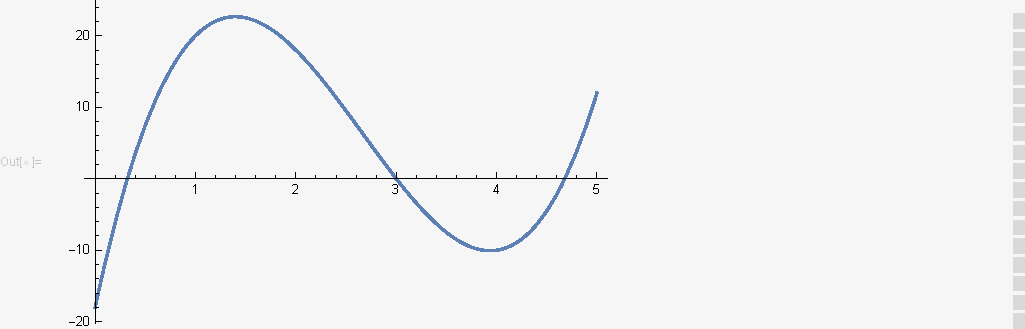
\includegraphics{HW_6_screenshots/q_2}
        \item
        f[\text{x$\_$},\text{u$\_$}]=\text{Total}[\text{Table}[D[\text{Sin}[u],\{u,i\}]/\text{Factorial}[i] x{}^{\wedge}i,\{i,0,20\}]]\\
        \text{Plot}[\{f[x,\text{Pi}]\},\{x,0,2 \text{Pi}\}]

        \begin{doublespace}
            \noindent\(x \text{Cos}[u]-\frac{1}{6} x^3 \text{Cos}[u]+\frac{1}{120} x^5 \text{Cos}[u]-\frac{x^7 \text{Cos}[u]}{5040}+\frac{x^9 \text{Cos}[u]}{362880}-\frac{x^{11}
                \text{Cos}[u]}{39916800}+\frac{x^{13} \text{Cos}[u]}{6227020800}-\frac{x^{15} \text{Cos}[u]}{1307674368000}+\frac{x^{17} \text{Cos}[u]}{355687428096000}-\frac{x^{19}
                \text{Cos}[u]}{121645100408832000}+\text{Sin}[u]-\frac{1}{2} x^2 \text{Sin}[u]+\frac{1}{24} x^4 \text{Sin}[u]-\frac{1}{720} x^6 \text{Sin}[u]+\frac{x^8
            \text{Sin}[u]}{40320}-\frac{x^{10} \text{Sin}[u]}{3628800}+\frac{x^{12} \text{Sin}[u]}{479001600}-\frac{x^{14} \text{Sin}[u]}{87178291200}+\frac{x^{16}
                \text{Sin}[u]}{20922789888000}-\frac{x^{18} \text{Sin}[u]}{6402373705728000}+\frac{x^{20} \text{Sin}[u]}{2432902008176640000}\)
        \end{doublespace}

        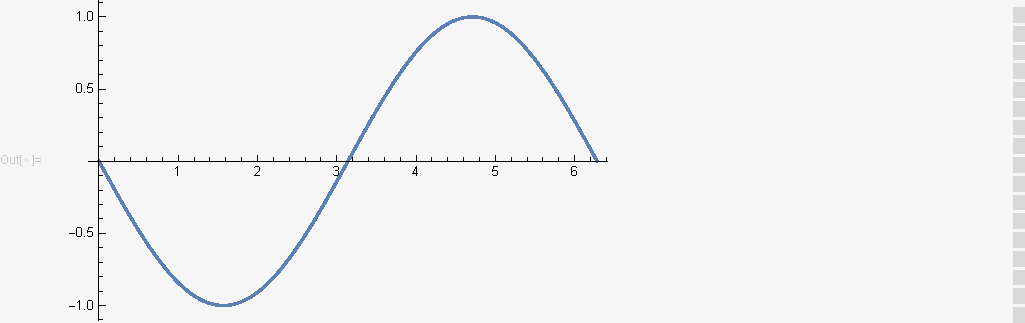
\includegraphics{HW_6_screenshots/q_3}
        \item
        A=\text{Table}[\text{Table}[\text{Sin}[i j], \{j,10\}], \{i, 10\}];\\
        b=\text{Table}[i,\{i,10\}];\\
        \text{LinearSolve}[N[A],N[b]]

        \begin{doublespace}
            \noindent\(\{2.83492,-5.65071,-16.77,-9.82246,2.24527,-5.75988,-2.63877,2.96037,25.6627,23.0544\}\)
        \end{doublespace}
        \item
        \begin{enumerate}
            \item
            \item[(b-d)]
            \text{Clear}[x,v,\text{energy},\text{dotenergy},\text{ndiv},\text{dt}];\\
            \text{ndiv}=2000;\\
            \text{dt}=N[(8 \text{Pi})/\text{ndiv}];\\
            v[\text{n$\_$}]\text{:=}v[n]=v[n-1]-x[n-1] \text{dt};\\
            v[0]=0;\\
            x[\text{n$\_$}]\text{:=}x[n]=x[n-1]+v[n-1] \text{dt};\\
            x[0]=1;\\
            \text{ListPlot}[\text{Table}[\{x[t],v[t]\},\{t,0,\text{ndiv}\}]]\\
            \text{energy}[\text{n$\_$}]\text{:=}\text{energy}[n]=(x[n]{}^{\wedge}2+v[n]{}^{\wedge}2)/2\\
            \text{ListPlot}[\text{Table}[\text{energy}[t],\{t,0,\text{ndiv}\}]]\\
            \text{dotenergy}[\text{n$\_$}]\text{:=}\text{dotenergy}[n]=(\text{energy}[n+1]-\text{energy}[n])/\text{dt}\\
            \text{ListPlot}[\text{Table}[\text{dotenergy}[t],\{t,0,\text{ndiv}\}]]

            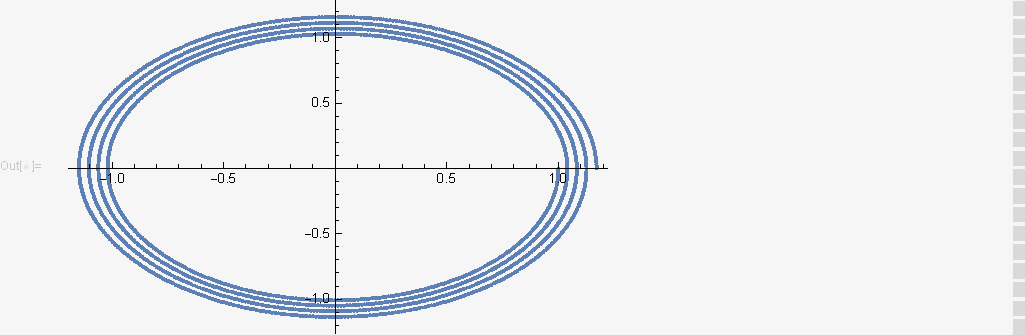
\includegraphics{HW_6_screenshots/q_5_gr1}

            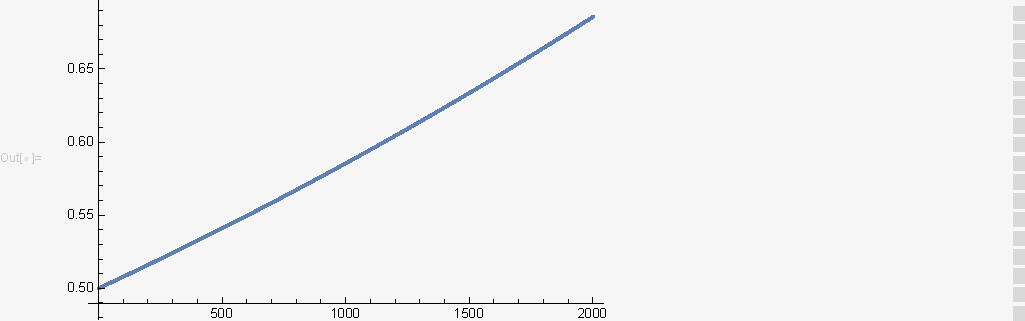
\includegraphics{HW_6_screenshots/q_5_gr2}

            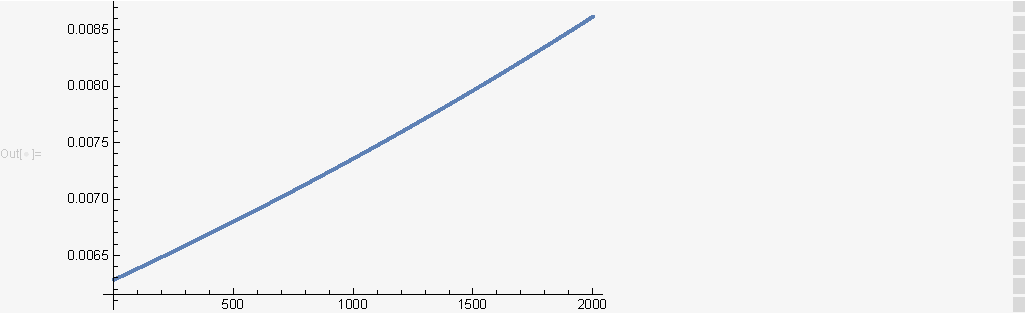
\includegraphics{HW_6_screenshots/q_5_gr3}



            \text{Clear}[x,v,\text{energy},\text{dotenergy},\text{ndiv},\text{dt}];\\
            \text{ndiv}=2000;\\
            \text{dt}=N[(8 \text{Pi})/\text{ndiv}];\\
            v[\text{n$\_$}]\text{:=}v[n]=v[n-1]-x[n-1] \text{dt};\\
            v[0]=0;\\
            x[\text{n$\_$}]\text{:=}x[n]=x[n-1]+v[n] \text{dt};\\
            x[0]=1;\\
            \text{ListPlot}[\text{Table}[\{x[t],v[t]\},\{t,0,\text{ndiv}\}]]\\
            \text{energy}[\text{n$\_$}]\text{:=}\text{energy}[n]=(x[n]{}^{\wedge}2+v[n]{}^{\wedge}2)/2\\
            \text{ListPlot}[\text{Table}[\text{energy}[t],\{t,0,\text{ndiv}\}]]\\
            \text{dotenergy}[\text{n$\_$}]\text{:=}\text{dotenergy}[n]=(\text{energy}[n+1]-\text{energy}[n])/\text{dt}\\
            \text{ListPlot}[\text{Table}[\text{dotenergy}[t],\{t,0,\text{ndiv}\}]]


            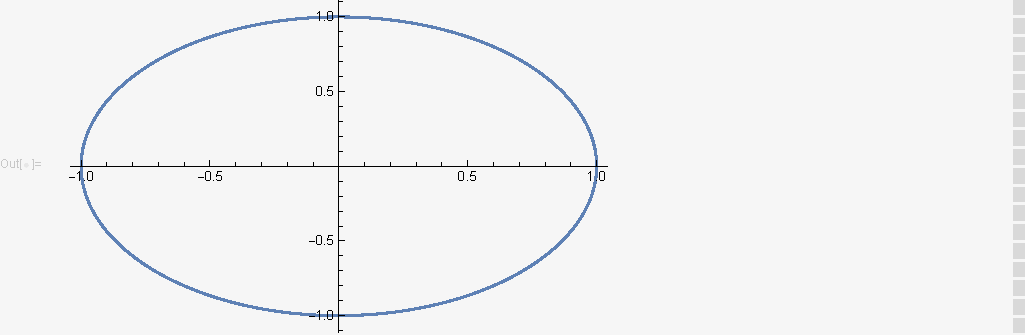
\includegraphics{HW_6_screenshots/q_5_gr4}

            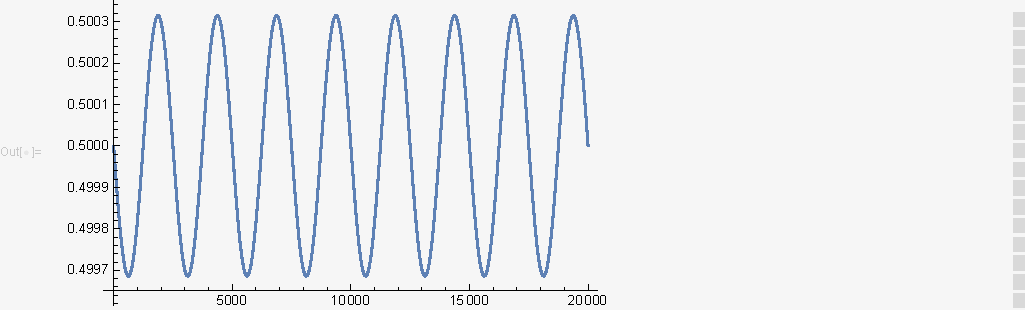
\includegraphics{HW_6_screenshots/q_5_gr5}

            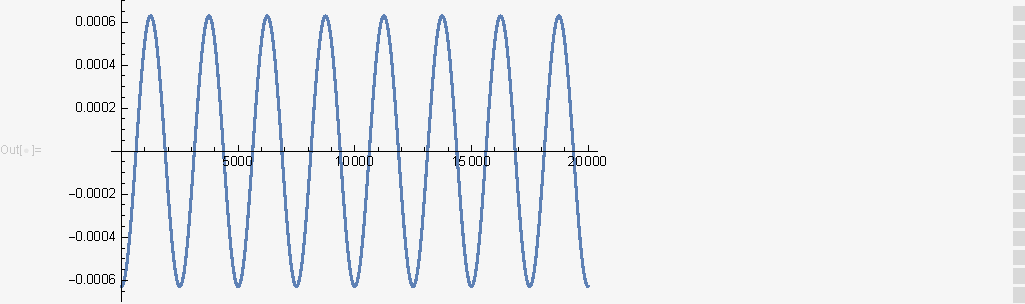
\includegraphics{HW_6_screenshots/q_5_gr6}

        \end{enumerate}
    \end{enumerate}

\end{document}